%--------------------------------------------------------------------------------------------------
\chapter{Umsetzung des Konzepts mit Hilfe der Unity Enginge}\label{cha:Umsetzung}
In diesem Kapitel wird die Umsetzung des Menschmodells und der Interaktion in der Entwicklungsumgebung der Unity Engine vorgestellt. Daher gibt es zunächst einen Einblick in die genutzte Hardware und Software, bevor das Menschmodell und die Interaktionsschnittstelle genauer erläutert werden.
%--------------------------------------------------------------------------------------------------
\section{Eingesetzte Hardware}\label{sec:Hardware}
Für die Umsetzung dieses Projektes wurde die Virtual Reality Brille \textbf{VIVE Pro} (Vgl. Abbildung \ref{fig:ViveproKit}) vom Hersteller HTC verwendet, da sie eine der Leistungsstärksten Brillen auf dem Markt ist. Zu den Stärken dieser Brille gehören das kontrastreiche OLED-Display, die sehr hohe Auflösung von 1440 x 1600 Pixeln pro Auge, eine Bildwiederholrate von 90Hz, ein Sichtfeld von 110 Grad und vor allem die Möglichkeit die Brille mit Hilfe des \textbf{Vive Wireless Sets} (Vgl. Abbildung \ref{fig:WirelessKit}) kabellos zu verwenden. Es ist anzumerken, dass für das kabellose Verwenden dieser VR Brille eine \textbf{Erweiterungskarte} in den PC eingebaut werden muss um einen speziellen \textbf{Empfänger} für die Signale der Brille anzuschließen. Des Weiteren muss ein \textbf{Sender} an der VR-Brille angebracht werden, welcher mit dem am PC angeschlossenen Empfänger kommuniziert und durch einen \textbf{mobilen Akku} mit Strom versorgt wird. Der mitgelieferte mobile Akku ermöglicht einen kabellosen Einsatz der VR Brille für bis zu sechs Stunden (Vgl. Abbildung \ref{fig:WirelessKit}) [28, ViveWeb].
\newline\newline
Um die Brille zu verwenden bedarf es mindesten zwei der sogenannten \textbf{SteamVR 2.0 Basisstationen} (Vgl. Abbildung \ref{fig:ViveproKit}), welche dem Bediener in Kombination mit des Vive Wireless Adapters eine enorme Bewegungsfreiheit ermöglichen. Beim Einsatz von zwei solcher Basisstationen ist eine Raumgröße von bis zu 5m x 5m, also 25m² möglich. Es ist sogar möglich bis zu vier solcher Basisstationen zu Verwenden und somit eine Raumgröße von bis zu 10m x 10m, also 100m² zu unterstützen [28, ViveWeb].
\newline\newline
Ein weiteres notwendiges Zubehör der Brille sind die beiden \textbf{Controller} (Vgl. Abbildung \ref{fig:ViveproKit}), die es dem Bediener ermöglichen mit der virtuellen Umgebung zu interagieren. Beide Controller werden wie die VR Brille durch die Basisstationen im Raum geortet und liefern Informationen über ihre eigene Position und Ausrichtung im Raum. Zusätzlich verfügen beide Controller über jeweils fünf Tasten, welche man mit eigenen Funktionalitäten versehen kann. Es ist anzumerken, dass die Tasten alle unterschiedlich sind und daher für unterschiedliche Zwecke verwendet werden können [29, ViveController].
\newline
Auf der Vorderseite der Controller befinden sich insgesamt drei Tasten [29, ViveController]:
\begin{itemize}
	\item Die erste dieser Tasten (ganz unten) ist die Taste um das Hauptmenü aufzurufen. Diese 
	Taste wird in der Regel nicht überschrieben und behält diese Funktionalität bei.
	\item Die zweite Taste (mittig) ist gleichzeitig ein Berührungsempfindliches Trackpad. Dem 
	Entwickler steht es frei, ob er diese Taste als einfache Taste oder als Trackpad verwenden 
	möchte. Es ist sogar Möglich beide Funktionen gleichzeitig in einer Anwendung zu 
	unterstützen. Dadurch eröffnen sich viele Anwendungsmöglichkeiten für diese Taste.
	\item Die dritte Taste (oben) ist wiederrum eine ganz einfache Taste und wird in den meisten 
	Anwendungen als eine einfache Menü-Taste verwendet.
\end{itemize}
Auf der Rückseite und der Außenseite des Controllers befinden sich zwei weitere Tasten [29, ViveController]:
\begin{itemize}
	\item Die Tasten links und rechts an der Außenseite des Controllers bilden eine Taste, welche 
	ausgelöst wird, wenn der Bediener den Controller fest mit der Hand drückt.
	\item Die Taste auf der Rückseite hat wie das Trackpad auf der Vorderseite zwei 
	Einsatzmöglichkeiten. Sie kann einerseits als einfache Taste verwendet werden, andererseits 
	als berührungsempfindlicher Auslöser, da der Entwickler über die Software-Schnittstelle 
	auslesen kann wie tief die Taste eingedrückt wurde, ähnlich wie bei einem Gaspedal in
	einem Auto.
\end{itemize}
\begin{figure}[h]
	\centering
	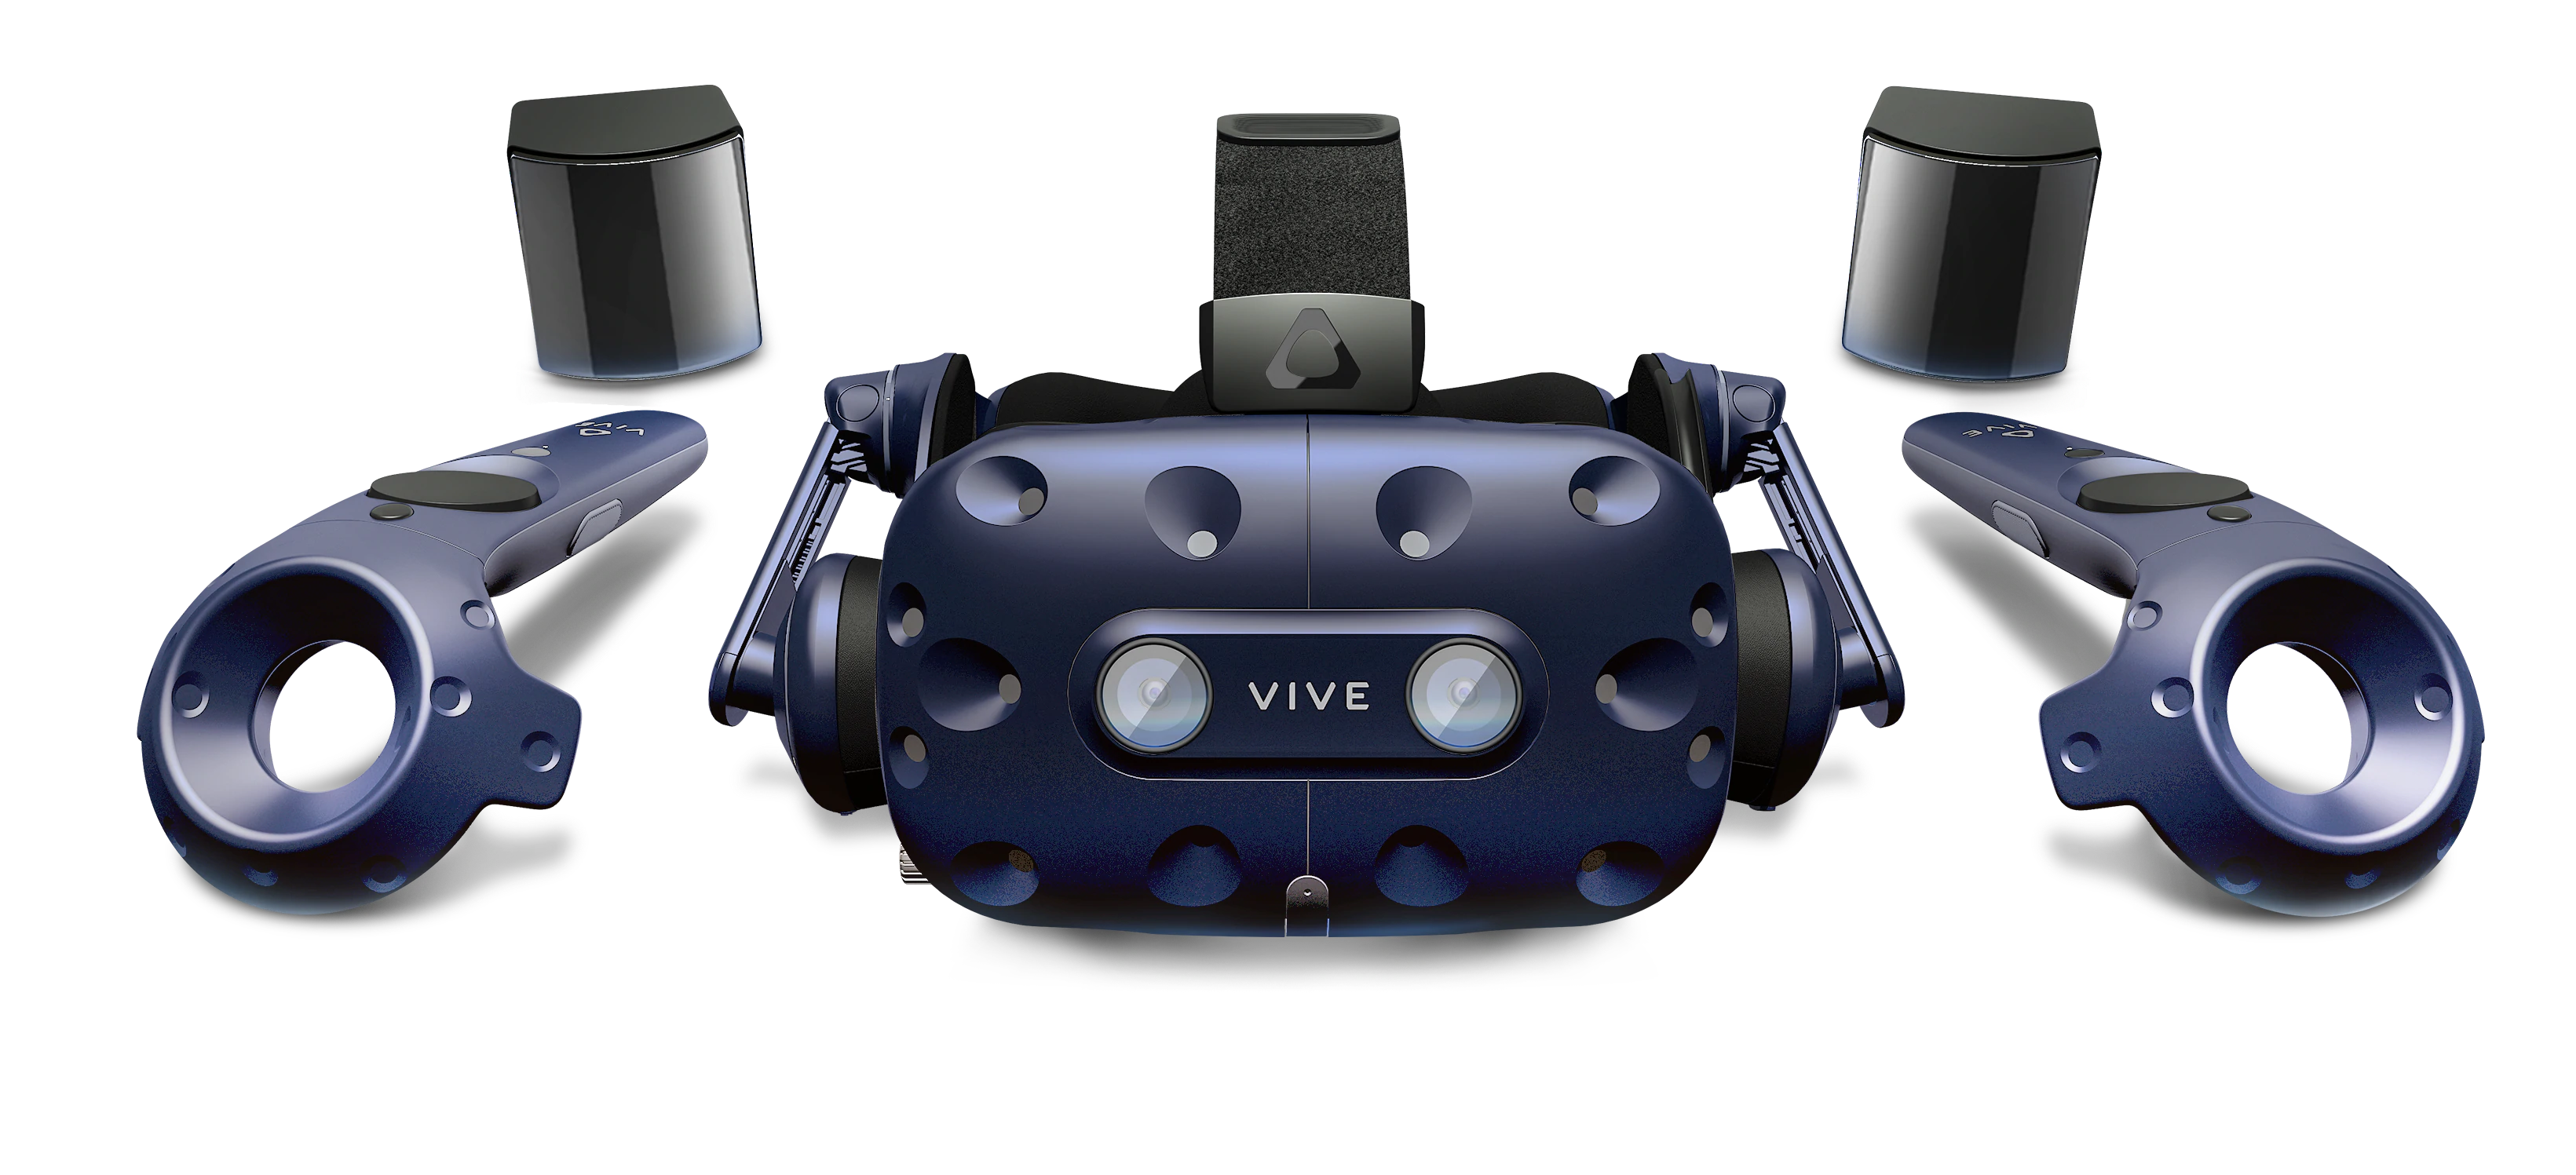
\includegraphics[width=0.7\linewidth]{Bilder/A26_Vivepro}
	\caption{VIVE Pro (mitte), Controller und Basisstationen (außen) [A26]}
	\label{fig:ViveproKit}
\end{figure}
\begin{figure}[h]
	\centering
	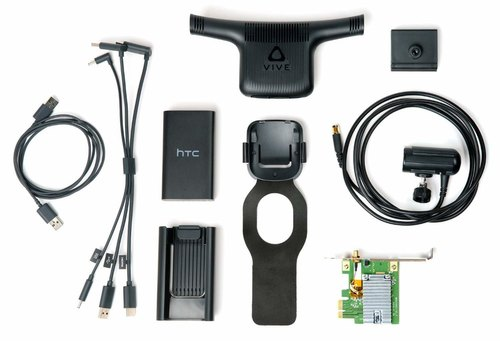
\includegraphics[width=0.5\linewidth]{Bilder/A27_WirelessKit}
	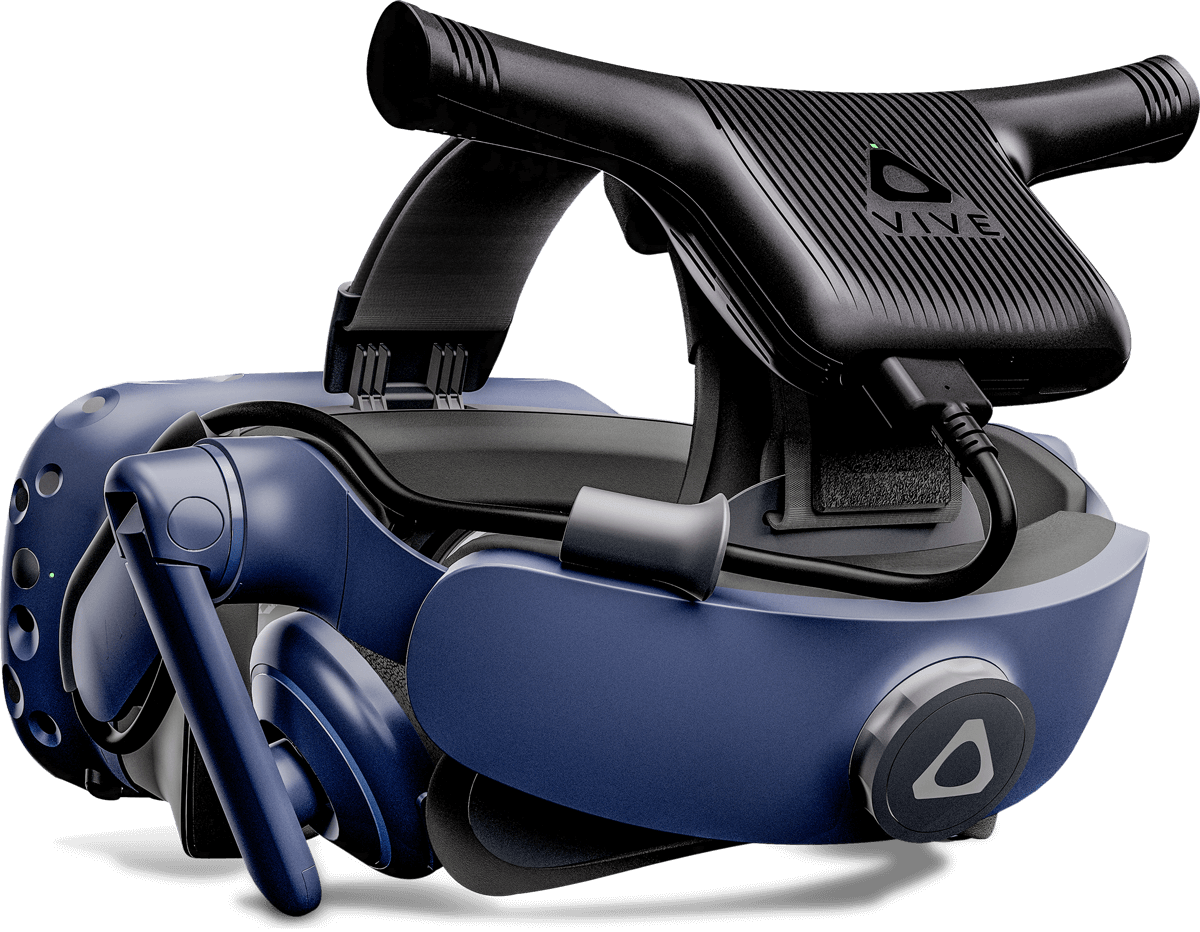
\includegraphics[width=0.4\linewidth]{Bilder/A28_Vive+Wireless}
	\caption{Links: VIVE Wireless Set, inkl. Erweiterungskarte, Sender, Empfänger, Akku, Kabeln und Befestigungen. Rechts: VR Brille mit angeschlossenem Sender. [A27+A28]}
	\label{fig:WirelessKit}
\end{figure}
Neben den außerordentlich guten technischen Spezifikationen der HTC VIVE Pro waren die \textbf{HTC VIVE Tracker} (Vgl. Abbildung \ref{fig:ViveTracker}) ein weiterer Grund warum diese VR Brille zur Umsetzung dieser Arbeit ausgewählt wurde. Die VIVE Tracker werden genauso wie die VR Brille und die dazugehörigen Controller von den Basisstationen im raum geortet und liefern ebenfalls Informationen über ihre Position und Ausrichtung im Raum. Durch den kleinen Formfaktor können die Tracker an beliebigen Objekten befestigt werden um die Bewegung dieser Objekte in der virtuellen Welt abzubilden [30, ViveTracker].
\newline
\begin{figure}[h]
	\centering
	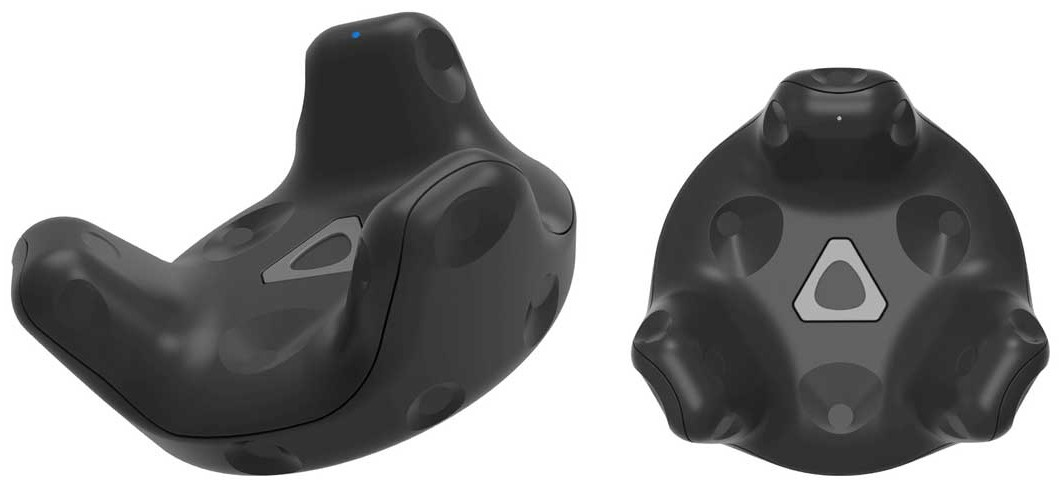
\includegraphics[width=0.5\linewidth]{Bilder/A29_ViveTracker}
	\caption{HTC VIVE Tracker [A29]}
	\label{fig:ViveTracker}
\end{figure}
\newline
Bei dieser Arbeit kamen die Tracker für die Ortung einzelner Körperteile zum Einsatz, da die Hände und der Kopf werden bereits durch die Controller und die VR Brille abgedeckt wurden. Konkret kamen die Tracker für die Ortung der Füße, der Knie, des Beckens und der Ellenbogen zum Einsatz. Durch das Schraubgewinde auf der Unterseite lassen sich die Tracker einfach befestigen. Für die Befestigungen am Becken und an den Füßen wurde auf \textbf{fertige Halterungen} zurückgegriffen (Vgl. Abbildung \ref{fig:Mounts}). Um die Tracker an den Knien und an den Ellenbogen zu befestigen habe ich mir \textbf{eigene Halterungen} gebaut (Vgl. Abbildung \ref{fig:Mounts}). Für diese Halterungen wurden handelsübliche Knie- und Ellenbogenschoner verwendet, durch die ein Loch gebohrt wurde um eine Schraube mit Hilfe einer Mutter zu fixieren. Durch das bereits erwähnte Schraubgewinde auf der Unterseite der Tracker ließen diese sich einfach an diesen Schrauben befestigen.
\begin{figure}[h]
	\centering
	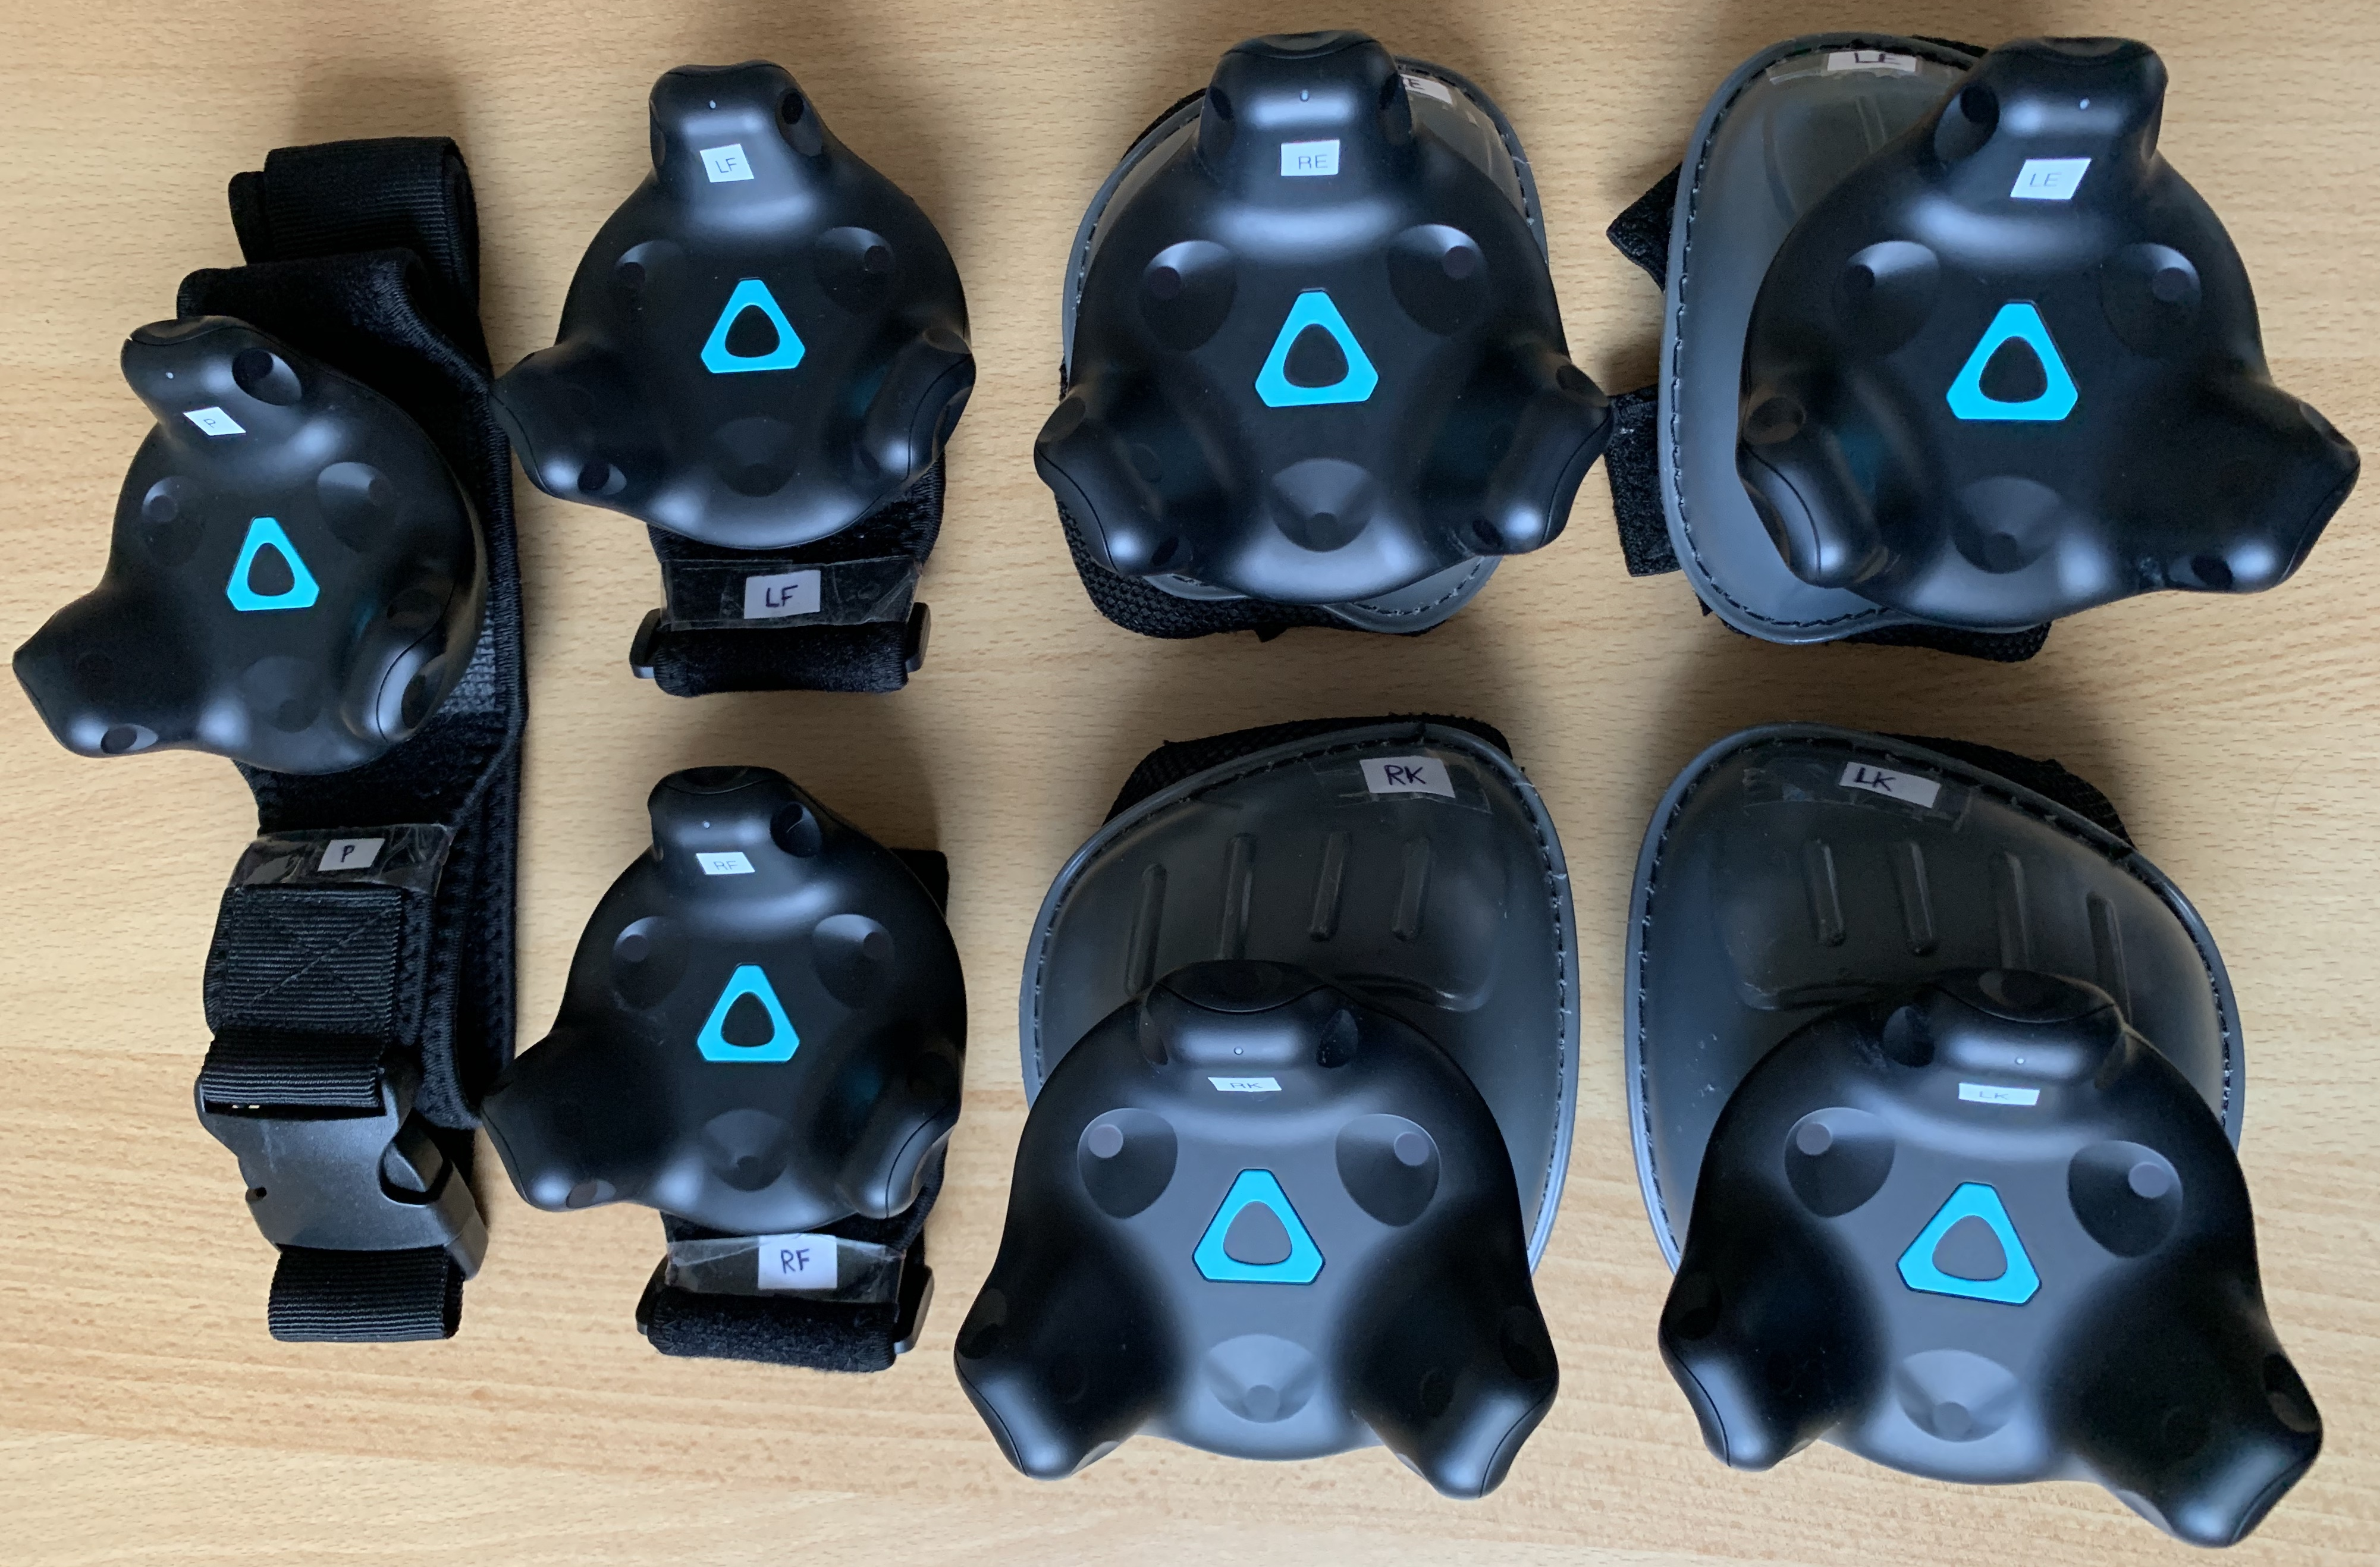
\includegraphics[width=0.7\linewidth]{Bilder/A32_Mounts}
	\caption{Gekaufte (links) und eigene (rechts) Befestigungen für die Tracker, eigene Abbildung}
	\label{fig:Mounts}
\end{figure}

%--------------------------------------------------------------------------------------------------
\section{Eingesetzte Software}\label{sec:Software}
